\hypertarget{_config_regs18f4520_8h}{\section{Config\+Regs18f4520.\+h File Reference}
\label{_config_regs18f4520_8h}\index{Config\+Regs18f4520.\+h@{Config\+Regs18f4520.\+h}}
}


Include file to set the Configuration Bits of a P\+I\+C18\+F4520.  


{\ttfamily \#include $<$p18cxxx.\+h$>$}\\*
Include dependency graph for Config\+Regs18f4520.\+h\+:\nopagebreak
\begin{figure}[H]
\begin{center}
\leavevmode
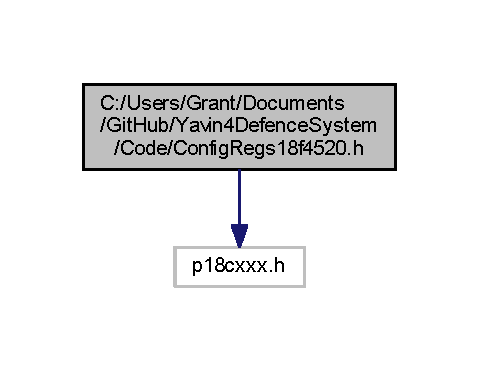
\includegraphics[width=188pt]{_config_regs18f4520_8h__incl}
\end{center}
\end{figure}


\subsection{Detailed Description}
Include file to set the Configuration Bits of a P\+I\+C18\+F4520. 

If the macro \+\_\+\+\_\+\+D\+E\+B\+U\+G is defined, the bits are set as appropriate for development and debugging\+:
\begin{DoxyItemize}
\item H\+S Oscillator; Oscillator Switch disabled; Power-\/\+On Timer;
\item Brown-\/out Reset disabled;
\item Watchdog Timer disabled;
\item C\+C\+P2 Multiplex disabled;
\item Stack Overflow Reset;
\item Low-\/voltage Programming disabled, Debug mode enabled;
\item No protection bits set.
\end{DoxyItemize}

If the macro \+\_\+\+\_\+\+D\+E\+B\+U\+G is N\+O\+T defined, the bits are set as appropriate for production code release\+:
\begin{DoxyItemize}
\item H\+S Oscillator; Oscillator Switch disabled; Power-\/\+On Timer;
\item Brown-\/out Reset enabled at 4.\+2\+V;
\item Watchdog Timer disabled;
\item C\+C\+P2 Multiplex disabled;
\item Stack Overflow Reset;
\item Low-\/voltage Programming and Debug mode disabled;
\item No protection bits set.
\end{DoxyItemize}

\begin{DoxyVersion}{Version}
0.\+1 -\/ derived from Config\+Regs18\+F452.\+h 
\end{DoxyVersion}
\begin{DoxyDate}{Date}
28-\/\+Aug-\/2014 
\end{DoxyDate}
\begin{DoxyAuthor}{Author}
David Rye
\end{DoxyAuthor}
\begin{DoxyNote}{Note}
This file was generated by the compiler from the command line\+: mcc18 -\/p18f4520 --help-\/config $>$ config\+Reg18\+F4520.\+h
\end{DoxyNote}
\begin{DoxyRefDesc}{Todo}
\item[\hyperlink{todo__todo000001}{Todo}]Consider if Watchdog Timer should be enabled for production code, and add W\+D\+T management code if so.\end{DoxyRefDesc}


\begin{DoxyRefDesc}{Todo}
\item[\hyperlink{todo__todo000002}{Todo}]Consider if Stack Overflow Reset should be enabled for production code. It may be better not to, as there is no re-\/entrant or recursive code, or dynamic memory allocation here -\/ if the code loads statically it should run.\end{DoxyRefDesc}


\begin{DoxyRefDesc}{Todo}
\item[\hyperlink{todo__todo000003}{Todo}]Change startup code c016iz.\+c so that everything (including initialised variables) correctly re-\/starts if \hyperlink{newmain_8c_acdef7a1fd863a6d3770c1268cb06add3}{main()} ever exits or a B\+O\+R or W\+D\+T reset occurs. \end{DoxyRefDesc}


Definition in file \hyperlink{_config_regs18f4520_8h_source}{Config\+Regs18f4520.\+h}.

